\taskpic{К концу однородной палочки массой $M = 4{,}4\mbox{ г}$
  подвешен на невесомой нити однородный алюминиевый шарик радиуса $r =
  0{,}5\mbox{ см}$. Палочку кладут на край стакана с водой, добиваясь
  такого положения равновесия, при котором погруженной в воду окажется
  половина шарика. Плотность алюминия равна $\rho_{\mbox{\textit{ал}}}
  = 2{,}7\cdot10^3\mbox{ кг/м}^3$, плотность воды
  $\rho_{\mbox{\textit{в}}} = 1\cdot10^3\mbox{ кг/м}^3$. Определите, в
  каком отношении $y/x$ делится длина палочки в этом случае. Объем
  шара радиуса $r$ равен $4\pi r^3/3$.}{
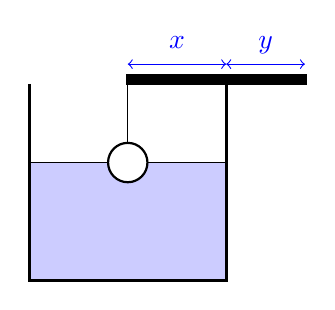
\begin{tikzpicture}
  \draw[fill=blue!20] (0,0.5) rectangle ++(2.5,1.5);
  \draw[very thick] (0,3) -- ++(0,-2.5) -- ++(2.5,0) -- ++(0,2.5);
  \draw[thick,fill=white] (1.25,2) circle (0.25);
  \draw (1.25,2.25) -- ++(0,0.75);
  \draw[very thick,fill=black] (1.25,3) rectangle ++(2.25,0.1);
  \draw[blue,<->] (1.25,3.25) -- ++(1.25,0) node[midway,above=2] {$x$};
  \draw[blue,<->] (2.5,3.25) -- ++(1,0) node[midway,above] {$y$};
\end{tikzpicture}
}